% Author: PokMan Ho pok.ho19@imperial.ac.uk
% Script: heatmap.tex
% Desc: heatmap section
% Input: none
% Output: none
% Arguments: 0
% Date: Apr 2020

\documentclass[../note.tex]{subfiles} %% use packages & commands as this main file

\begin{document}

\section{2D level plot (heatmap) with given data}
Heatmap is available for ``stats" package\autocite{Rcore}, which requires a matrix input and without a intrinsic colour reference (forum \href{https://stackoverflow.com/questions/9314658/colorbar-from-custom-colorramppalette}{thread} on creating a colour reference).  ``ggplot2" package\autocite{ggplot} also provide a \href{https://stackoverflow.com/questions/43772017/continuous-gradient-color-fixed-scale-heatmap-ggplot2}{solution} but the code is long.  For users not used to the ``ggplot2" package, the learning curve for you might be steep.  Hence, I recommend the ``lattice" package\autocite{lattice}, which provides a simple yet on-point method for plotting a dependent variable against two independent variables.

Below is a feature comparison table of the above three candidates, which showed the optimal efficiency can be obtained by using the ``lattice" package.
\begin{center}
    \begin{tabular}{r|ccc}\hline
        & ``lattice" & ``stats" & ``ggplot2" \\\hline
        \begin{tabular}{r}
            command\\name
        \end{tabular} & \href{https://www.rdocumentation.org/packages/lattice/versions/0.10-10/topics/levelplot}{levelplot} & \href{https://www.rdocumentation.org/packages/stats/versions/3.6.2/topics/heatmap}{heatmap} & \href{https://www.rdocumentation.org/packages/ggplot2/versions/3.3.0/topics/geom_raster}{geom\_raster} / \href{https://www.rdocumentation.org/packages/ggplot2/versions/3.3.0/topics/geom_raster}{geom\_tile}\\
        input &
        \begin{tabular}{|ccc|}\hline
            x & y & z \\\hline
            x1 & y1 & z11 \\
            x1 & y2 & z12 \\
            $\vdots$ & $\vdots$ & $\vdots$ \\
            x2 & y1 & z21 \\
            x2 & y2 & z22 \\
            $\vdots$ & $\vdots$ & $\vdots$ \\
            x$_n$ & y$_{n-1}$ & z$_{nn-1}$ \\
            x$_n$ & y$_n$ & z$_{nn}$ \\
        \hline\end{tabular}
        &
        \begin{tabular}{|c|cccc|}\hline
            & x1 & x2 & $\vdots$ & x$_n$ \\\hline
            y1 & z11 & z21 & $\vdots$ & zn1 \\
            y2 & z12 & z22 & $\vdots$ & zn2 \\
            $\vdots$ & $\vdots$ & $\vdots$ & $\ddots$ & $\vdots$ \\
            y$_{n-1}$ & z$_{1n-1}$ & z$_{2n-1}$ & $\vdots$ & z$_{nn-1}$ \\
            y$_n$ & z$_{1n}$ & z$_{2n}$ & $\vdots$ & z$_{nn}$ \\
        \hline\end{tabular}
        &
        \begin{tabular}{|ccc|}\hline
            x & y & z \\\hline
            x1 & y1 & z11 \\
            x1 & y2 & z12 \\
            $\vdots$ & $\vdots$ & $\vdots$ \\
            x2 & y1 & z21 \\
            x2 & y2 & z22 \\
            $\vdots$ & $\vdots$ & $\vdots$ \\
            x$_n$ & y$_{n-1}$ & z$_{nn-1}$ \\
            x$_n$ & y$_n$ & z$_{nn}$ \\
        \hline\end{tabular}\\
        \begin{tabular}{r}
            default\\colour scale
        \end{tabular} & yes & no & yes\\
        \begin{tabular}{r}
            default\\accessory
        \end{tabular} & no & \begin{tabular}{l}
            dendrogram,\\row-/column-wise colourbar
        \end{tabular} & no\\
    \hline\end{tabular}
\end{center}

One thing to note is ``missing data", which would always being displayed as ``white" in the levelplots (Fig.\ref{g:lv3}).  So do avoid having this colour as part of the colour scale to prevent confusions.

\subsection{continuous numeric}
\begin{code}
set.seed(998)\\
\# fix random number algorithm for code reproducibility\\\\
y=c()\\
\# initialise column\\\\
for(i in -3:6){y<-c(y,rep(i,10))}\\
\# fill in the column with repeated numbers (every number is repeated 10 times) from -3 to 6\\\\
rm(i)\\
\# remove token remnant from the loop for clarity (optional)\\\\
c0 = data.frame("x"=rep(-5:4,10), "y"=y, "z"=runif(100)-.5)\\
\# construct a three-columned dataframe "c0"\\
\# column names are "x", "y", "z" respectively\\
\# column "x" is a number sequence -5 to 4 repeated by 10 times\\
\# column "y" is the \textbf{y} column variable above\\
\# column "z" is a chain of 100 random numbers ranged from -0.5 to +0.5 (default range is from 0 to 1)\\\\
rm(y)\\
\# remove leftover column material for clarity (optional)
\end{code}

\begin{code}
library(lattice)\\\\
levelplot(c0\$z~c0\$x*c0\$y, col.regions = rev(gray(20:70/100)), xlab = "x-axis", ylab = "y-axis", main="levelplot from dataframe c0")\\\\
\# this is a levelplot with z-column ("c0\$z") plotting against the interacting ("*") x-axis ("c0\$x") and y-axis ("c0\$y")\\
\# we use gray-scale ("gray") from 20\% to 70\% with lighter colour at bottom ("rev")\\
\# we then name the x-axis title ("xlab"), y-axis title ("ylab") and figure title ("main") as some desired text-string
\end{code}

\begin{figure}[H]
    \centering
    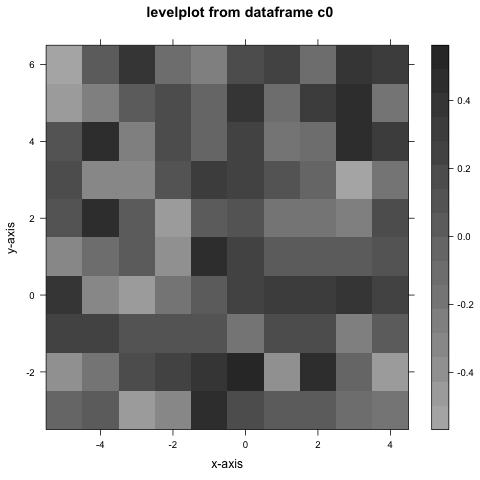
\includegraphics[width=.5\linewidth]{graph/lvPlt1.png}
    \label{g:lv1}
\end{figure}

\subsection{unordered categorical}
\begin{code}
set.seed(998)\\\\
c1 = data.frame("x"=c("A","B","C"), "y"=c(rep("A",3), rep("B",3), rep("C",3)), "z"=runif(9)-.2)\\
\# a three-columned dataframe named "c1" with column names "x", "y", "z"\\
\# column "x" is a chain of 3-elements textstring\\
\# column "y" is a chain of repeated character textstring\\
\# column "z" is a random number chain of nine numbers ranged from -0.2 to +0.8\\
\# when constructing the dataframe, element chain in column "y" and "z" have lengths divisible by that of column "x"; so the column "x" will be reused in sequence
\end{code}

\begin{code}
library(lattice)\\\\
levelplot(c1\$z~c1\$x*c1\$y, col.regions = rev(gray(10:80/100)), xlab = "x-axis", ylab = "y-axis", main="levelplot from dataframe c1")\\\\
\# this code is same as the one for Fig.\ref{g:lv1} except modifying the data source, greyscale range and figure title
\end{code}

\begin{figure}[H]
    \centering
    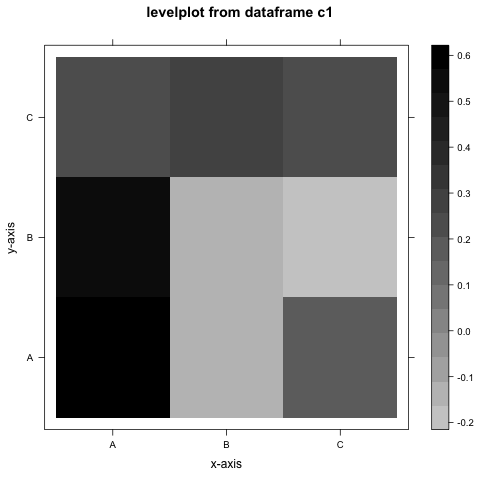
\includegraphics[width=.5\linewidth]{graph/lvPlt2.png}
    \label{g:lv2}
\end{figure}

\subsection{mixed datatypes}
\begin{code}
set.seed(998)\\\\
c2 = data.frame("x"=rep(-1:1,3), "y"=c(rep("A",3), rep("B",3), rep("C",2),"D"), "z"=runif(9)-.2)\\
\# this is a similar dataframe mixing the above two dataframe datatype characteristics\\
\# the only difference is this time we introduced a new category "D" to replace the last element under category "C"
\end{code}

\begin{code}
library(lattice)\\\\
levelplot(c2\$z~c2\$x*c2\$y, col.regions = rev(gray(30:50/100)), xlab = "x-axis", ylab = "y-axis", main="levelplot from dataframe c2")\\\\
\# this code is same as the one for Fig.\ref{g:lv1} except modifying the data source, greyscale range and figure title
\end{code}

\begin{figure}[H]
    \centering
    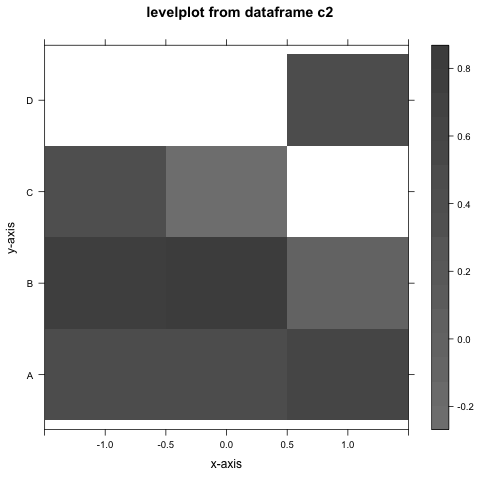
\includegraphics[width=.5\linewidth]{graph/lvPlt3.png}
    \label{g:lv3}
\end{figure}

\end{document}